\documentclass{ximera}

% These macros are automatically generated from the "macros"
% XML element.  Make permanent edits there.
%
% History
%   2004/01/01  Initiated for FCLA, evolved from there
%   2006/09/17  Converted  _, ^  to \sb, \sp for TeX4ht
%   2014/02/01  Updated for MathBook XML projects
%               Obsolete in FCLA: \codeindent, \computerfont, \define
%               Change: MathJax wants \lt, so replaced by \lteval
%   2014/02/22  New: \orderof, \reals, \per
%   2015/08/16  Incorporated into MathBook XML version of FCLA
%
%%%%%%%%%%%%%%%%%%%%%
%
%     Conveniences
%
%%%%%%%%%%%%%%%%%%%%%
%
%  Order of (asymptotically limit of fraction is 1)
%  Usage: \orderof{some function}
%
\newcommand{\orderof}[1]{\sim #1}
%
%  Integers
%  Usage:  \Z
\newcommand{\Z}{\mathbb{Z}}
%
%  Real numbers, as set of scalars
%  Usage:  \reals
\newcommand{\reals}{\mathbb{R}}
%
%  n-space over real field
%  Usage: \complex{integer-dimension}
\newcommand{\real}[1]{\mathbb{R}^{#1}}
%
%  Complex numbers, as set of scalars
%  Usage:  \complexes
\newcommand{\complexes}{\mathbb{C}}
%
%  n-space over complex field
%  Usage: \complex{integer-dimension}
\newcommand{\complex}[1]{\mathbb{C}^{#1}}
%
%  Complex conjugation (scalar, vector, matrix)
%  Usage: \conjugate{object}
\newcommand{\conjugate}[1]{\overline{#1}}
%
%  Complex number modulus
%  Usage: \modulus{a+bi}
%  Presumes math mode
\newcommand{\modulus}[1]{\left\lvert#1\right\rvert}
%
%  Zero vector
%  Usage: \zerovector
\newcommand{\zerovector}{\vect{0}}
%
%  Zero matrix
%  Usage: \zeromatrix, use a subscript when size is important
\newcommand{\zeromatrix}{\mathcal{O}}
%
%  Inner product (brackets, not quadratic form)
%  Usage: \innerproduct{a-vector}{a-vector}
\newcommand{\innerproduct}[2]{\left\langle#1,\,#2\right\rangle}
%
%  Norm of a vector
%  Usage: \norm{a-vector}
\newcommand{\norm}[1]{\left\lVert#1\right\rVert}
%
%  Dimension
%  Usage: \dimension{vector-space-letter}
\newcommand{\dimension}[1]{\dim\left(#1\right)}
%
%  Nullity
%  Usage: \nullity{matrix-or-lintrans-letter}
\newcommand{\nullity}[1]{n\left(#1\right)}
%
%  Rank
%  Usage: \rank{matrix-or-lintrans-letter}
\newcommand{\rank}[1]{r\left(#1\right)}
%
%  Direct sum
%  Usage: \ds between a couple of subspaces
%
\newcommand{\ds}{\oplus}
%
%  Determinant of a matrix (functional)
%  Usage: \detname{A}
\newcommand{\detname}[1]{\det\left(#1\right)}
%
%  Determinant of a matrix (vertical bars)
%  Usage: \detbars{A}
\newcommand{\detbars}[1]{\left\lvert#1\right\rvert}
%
%  Trace of a Matrix
%  Usage: \trace{matrix name}
\newcommand{\trace}[1]{t\left(#1\right)}
%
%  Square Root of a Matrix
%  Usage: \sr{a-matrix}
\newcommand{\sr}[1]{#1^{1/2}}
%
%%%%%%%%%%%%%%%%%%%%%
%
%     Subspace Constructions
%
%%%%%%%%%%%%%%%%%%%%%
%
%  Span of a set of vectors
%  \span and \sp are used by TeX for other things
%  Usage: \spn{set-of-vectors}
\newcommand{\spn}[1]{\left\langle#1\right\rangle}
%
%  Null space of a matrix
%  Usage:  \nsp{A}
\newcommand{\nsp}[1]{\mathcal{N}\!\left(#1\right)}
%
%  Column space of a matrix
%  Usage:  \csp{A}
\newcommand{\csp}[1]{\mathcal{C}\!\left(#1\right)}
%
%  Row space of a matrix
%  Usage:  \rsp{A}
\newcommand{\rsp}[1]{\mathcal{R}\!\left(#1\right)}
%
%  Left null space of a matrix
%  Usage:  \lns{A}
\newcommand{\lns}[1]{\mathcal{L}\!\left(#1\right)}
%
%  Orthogonal complement of a vector space
%  Avoiding TeX's \perp
%  Usage:  \per{A}
\newcommand{\per}[1]{#1^\perp}
%
%%%%%%%%%%%%%%%%%%%%%
%
%     Systems of Equations
%
%%%%%%%%%%%%%%%%%%%%%
%
%  In-line form of an augmented matrix for a system of equations
%  Usage: \augmented{coefficient-matrix}{constant-vector}
\newcommand{\augmented}[2]{\left\lbrack\left.#1\,\right\rvert\,#2\right\rbrack}
%
%  Notation for a linear system before introducing matrix multiplication
%  Usage: \linearsystem{coefficient-matrix}{constant-vector}
\newcommand{\linearsystem}[2]{\mathcal{LS}\!\left(#1,\,#2\right)}
%
%  Notation for a homogenous system before introducing matrix multiplication
%  Usage: \homosystem{coefficient-matrix}
\newcommand{\homosystem}[1]{\linearsystem{#1}{\zerovector}}
%
%%%%%%%%%%%%%%%%%%%%%
%
%     Row Operations, Echelon Form
%
%%%%%%%%%%%%%%%%%%%%%
%
% Row operations on matrices
%
% Three commands to shorten up descriptions of gaussian elimination
%
% Usage: \rowopswap{row-i}{row-j}
% Usage: \rowopmult{scalar}{row-i}
% Usage: \rowopadd{scalar}{row-multiplied}{row-added-to}
\newcommand{\rowopswap}[2]{R_{#1}\leftrightarrow R_{#2}}
\newcommand{\rowopmult}[2]{#1R_{#2}}
\newcommand{\rowopadd}[3]{#1R_{#2}+R_{#3}}
%
% Mark leading 1's in echelon form with fbox
% Usage: \leading{a-1-usually}
\newcommand{\leading}[1]{\fbox{#1}}
%
%  Row-reduce arrow
%  Usage:  \rref inbetween a matrix and its reduced row-echelon form
\newcommand{\rref}{\xrightarrow{\text{RREF}}}
%
%  Elementary Matrices
%  Usage: \elemswap{subscript}{subscript}
%  Usage: \elemmult{scalar}{subscript}
%  Usage: \elemadd{scalar}{subscript-mult}{subscript-target}
%
\newcommand{\elemswap}[2]{E_{#1,#2}}
\newcommand{\elemmult}[2]{E_{#2}\left(#1\right)}
\newcommand{\elemadd}[3]{E_{#2,#3}\left(#1\right)}
%
%%%%%%%%%%%%%%%%%%%%%
%
%     2-D Constructions (Lists, Vectors, Matrices)
%
%%%%%%%%%%%%%%%%%%%%%
%
%  A list of scalars of generic length
%  Usage:  \scalarlist{scalar letter}{terminal subscript}
\newcommand{\scalarlist}[2]{{#1}_{1},\,{#1}_{2},\,{#1}_{3},\,\ldots,\,{#1}_{#2}}
%
%  Vector styling, bold (or use wiggles, arrows, whatever)
%  Subscripts go outside this construction
%  Usage: \vect{a symbol to use as a vector}
%  Have to already be in math mode
%
\newcommand{\vect}[1]{\mathbf{#1}}
%
%  A column vector
%  Usage: \colvector{list-delimited-by-\\}
%
\newcommand{\colvector}[1]{\begin{bmatrix}#1\end{bmatrix}}
%
%  A generic vector with components
%  Usage: \vectorcomponents{component-letter}{final-subscript}
\newcommand{\vectorcomponents}[2]{\colvector{#1_{1}\\#1_{2}\\#1_{3}\\\vdots\\#1_{#2}}}
%
%  A list of vectors of generic length
%  Usage:  \vectorlist{vector letter}{terminal subscript}
\newcommand{\vectorlist}[2]{\vect{#1}_{1},\,\vect{#1}_{2},\,\vect{#1}_{3},\,\ldots,\,\vect{#1}_{#2}}
%
%  Vector entries, entry i of vector v
%  (vector-expession still needs \vect, etc.)
%  Usage:  \vectorentry{vector-expression}{single-subscript}
\newcommand{\vectorentry}[2]{\left\lbrack#1\right\rbrack_{#2}}
%
%  Matrix entries, entry i,j of matrix A
%  Usage:  \matrixentry{matrix-expression}{paired-subscripts}
%
\newcommand{\matrixentry}[2]{\left\lbrack#1\right\rbrack_{#2}}
%
%  A generic linear combination
%  Usage:  \lincombo{scalar letter}{vector letter}{terminal subscript}
\newcommand{\lincombo}[3]{#1_{1}\vect{#2}_{1}+#1_{2}\vect{#2}_{2}+#1_{3}\vect{#2}_{3}+\cdots +#1_{#3}\vect{#2}_{#3}}
%
%  Matrix, column by column, as vectors
%  Usage:  \matrixcolumns{matrix letter}{terminal subscript}
\newcommand{\matrixcolumns}[2]{\left\lbrack\vect{#1}_{1}|\vect{#1}_{2}|\vect{#1}_{3}|\ldots|\vect{#1}_{#2}\right\rbrack}
%
%%%%%%%%%%%%%%%%%%%%%
%
%     Special Matrices
%
%%%%%%%%%%%%%%%%%%%%%
%
%  Transpose of a matrix
%  Usage:  \transpose{A}
\newcommand{\transpose}[1]{#1^{t}}
%
%  Inverse of a matrix
%  Usage:  \inverse{A}
\newcommand{\inverse}[1]{#1^{-1}}
%
%  Submatrix (for minors, determinants)
%  Usage: \submatrix{matrix-name}{delete-row}{delete-col}
\newcommand{\submatrix}[3]{#1\left(#2|#3\right)}
%
%  Adjoint of a matrix (twice)
%  This macro is a convenience to call \transpose and \conjugate properly
%  It shouldn't need to be modified (or mathematical meanings will change)
%  Usage:  \adj{A}
\newcommand{\adj}[1]{\transpose{\left(\conjugate{#1}\right)}}
%
%  This macro controls the symbol used for the adjoint
%  It can be edited to taste
%  Usage:  \adjoint{A}
\newcommand{\adjoint}[1]{#1^\ast}
%
%%%%%%%%%%%%%%%%%%%%%
%
%     Sets
%
%%%%%%%%%%%%%%%%%%%%%
%
%  A convenience for simple sets
%  Usage:  \set{list of element}
\newcommand{\set}[1]{\left\{#1\right\}}
%
%  Sets with vertical bar, "such that", sized for objects, not condition
%  Usage:  \setparts{objects}{condition}
%
%%\newcommand{\setparts}[2]{\left\{ #1\mid#2\right\}}
%%\newcommand{\setparts}[2]{\left\{\left. #1\right\rvert#2\right\}}
\newcommand{\setparts}[2]{\left\lbrace#1\,\middle|\,#2\right\rbrace}
%
%  Set Cardinality
%  Usage:  \card{a-set-letter}
\newcommand{\card}[1]{\left\lvert#1\right\rvert}
%
%  Set Union
%  Use \cup
%
%  Set Intersection
%  Use \cap
%
%  Set Complement
%  Usage:  \setcomplement{a-set-letter}
\newcommand{\setcomplement}[1]{\overline{#1}}
%
%%%%%%%%%%%%%%%%%%%%%
%
%     Eigenvalues and Eigenspaces
%
%%%%%%%%%%%%%%%%%%%%%
%
%  Characteristic polynomial
%  Usage: \charpoly{matrix-letter}{variable-letter}
\newcommand{\charpoly}[2]{p_{#1}\left(#2\right)}
%
%  Eigenspace
%  Usage: \eigenspace{matrix-letter}{eigenvalue-letter}
\newcommand{\eigenspace}[2]{\mathcal{E}_{#1}\left(#2\right)}
%
%  2013/10/03 Including ampersands is problematic here, 
%  think about fixes later
%  2014/02/22 Limited testing, seems &amp; is fine for HTML and LaTeX
%  2016-07-20 only employed in Archetypes, MBX has gather/align override
%  Eigensystem (presumes wrapped in an mrow within md)
%  Usage: \eigensystem{matrixletter}{eigenvalue}{list of basis vectors}
\newcommand{\eigensystem}[3]{\lambda&amp;=#2&amp;\eigenspace{#1}{#2}&amp;=\spn{\set{#3}}} 
%
%  Generalized Eigenspace
%  Usage: \geneigenspace{lin-trans-letter}{eigenvalue-letter}
\newcommand{\geneigenspace}[2]{\mathcal{G}_{#1}\left(#2\right)}
%
%  Algebraic multiplicty
%  Usage: \algmult{matrix-letter}{eigenvalue-letter}
\newcommand{\algmult}[2]{\alpha_{#1}\left(#2\right)}
%
%  Geometric multiplicty
%  Usage: \geomult{matrix-letter}{eigenvalue-letter}
\newcommand{\geomult}[2]{\gamma_{#1}\left(#2\right)}
%
%  Index (of eigenvalue)
%  Usage: \indx{matrix-letter}{eigenvalue-letter}
\newcommand{\indx}[2]{\iota_{#1}\left(#2\right)}
%
%%%%%%%%%%%%%%%%%%%%%
%
%     Linear Transformations
%
%%%%%%%%%%%%%%%%%%%%%
%
%  MathJax defines \lt to ease XML confusion
%
%  Linear transformation definition
%  Usage: \ltdefn{name-letter}{domain}{range}
\newcommand{\ltdefn}[3]{#1\colon #2\rightarrow#3}
%
%  Linear transformation evaluation
%  Usage: \lteval{name-letter}{input}
%  Replaces old \lt desired by MathJax
\newcommand{\lteval}[2]{#1\left(#2\right)}
%
% Linear transformation inverse
%  Usage: \ltinverse{name-letter}
\newcommand{\ltinverse}[1]{#1^{-1}}
%
%  Linear transformation restriction
%  Usage: \restrict{name-letter}{subspace-letter}
\newcommand{\restrict}[2]{{#1}|_{#2}}
%
%  Linear transformation preimage
%  Usage: \preimage{name-letter}{codomain-element}
\newcommand{\preimage}[2]{#1^{-1}\left(#2\right)}
%
%  Range of a linear transformation
%  TeX uses \range for something else
%  Usage:  \rng{T}
\newcommand{\rng}[1]{\mathcal{R}\!\left(#1\right)}
%
%  Kernel of a linear transformation
%  TeX uses \ker to do something different
%  Usage:  \krn{T}
\newcommand{\krn}[1]{\mathcal{K}\!\left(#1\right)}
%
%  Linear transformation composition
%  Usage: \compose{function-name}{function-name}
\newcommand{\compose}[2]{{#1}\circ{#2}}
%
%  Vector space of linear transformations
%  Usage: \vslt{domains}{codomains}
%  Presumes math mode
\newcommand{\vslt}[2]{\mathcal{LT}\left(#1,\,#2\right)}
%
%%%%%%%%%%%%%%%%%%%%%
%
%     Vector and Matrix Representations
%
%%%%%%%%%%%%%%%%%%%%%
%
%  Isomorphism symbol
%  Usage: \isomorphic
\newcommand{\isomorphic}{\cong}
%
%  Similarity
%  Usage: \similar{inner-matrix}{outer-invertible-matrix}
%  Rearranging this will not "fix" all desired changes throughout
%
\newcommand{\similar}[2]{\inverse{#2}#1#2}
%
%  Vector representation function name
%  Usage: \vectrepname{basis-letter}
\newcommand{\vectrepname}[1]{\rho_{#1}}
%
%  Vector representation output
%  Usage: \vectrep{basis-letter}{input}
\newcommand{\vectrep}[2]{\lteval{\vectrepname{#1}}{#2}}
%
%  Vector representation inverse function name
%  (Added later, not used consistently in FCLA)
%  Usage: \vectrepinvname{basis-letter}
\newcommand{\vectrepinvname}[1]{\ltinverse{\vectrepname{#1}}}
%
%  Vector representation inverse output
%  Usage: \vectrepinv{basis-letter}{input}
\newcommand{\vectrepinv}[2]{\lteval{\ltinverse{\vectrepname{#1}}}{#2}}
%
%  Matrix representation
%  Usage: \matrixrep{transformation-letter}{domain-basis-letter}{codomain-basis-letter}
\newcommand{\matrixrep}[3]{M^{#1}_{#2,#3}}
%
%  Matrix representation column-by-colum
%  2016-07-20 only employed once?
%  Usage: \matrixrepcolumns{transformation-letter}{codomain-basis-letter}{codomain-basis-vector-letter}{final-index}
\newcommand{\matrixrepcolumns}[4]{\left\lbrack \left.\vectrep{#2}{\lteval{#1}{\vect{#3}_{1}}}\right|\left.\vectrep{#2}{\lteval{#1}{\vect{#3}_{2}}}\right|\left.\vectrep{#2}{\lteval{#1}{\vect{#3}_{3}}}\right|\ldots\left|\vectrep{#2}{\lteval{#1}{\vect{#3}_{#4}}}\right.\right\rbrack}
%
%  Change of basis matrix
%  Usage: \cbm{domain-basis-letter}{codomain-basis-letter}
\newcommand{\cbm}[2]{C_{#1,#2}}
%
%%%%%%%%%%%%%%%%%%%%%
%
%     Canonical Forms
%
%%%%%%%%%%%%%%%%%%%%%
%
%  Jordan blocks
%  Usage: \jordan{size}{diagonal-element}
\newcommand{\jordan}[2]{J_{#1}\left(#2\right)}
%
%%%%%%%%%%%%%%%%%%%%%
%
%     Hadamard Matrices
%     Contributed by Elizabeth Million
%
%%%%%%%%%%%%%%%%%%%%%
%
%  Hadamard Product
%  Usage: \hadamard{a-matrix}{a-matrix}
\newcommand{\hadamard}[2]{#1\circ #2}
%
%  Hadamard identity matrix
%  Usage: \hadamardidentity{paired-subscripts-size-of-matrix}
\newcommand{\hadamardidentity}[1]{J_{#1}}
%
%  Hadamard inverse matrix
%  Usage: \hadamardinverse{matrix-expression}
\newcommand{\hadamardinverse}[1]{\widehat{#1}}


\title{Examples of Surjective Linear Transformations}

\begin{document}
\begin{abstract}
  We consider examples of surjective linear transformations, as well as examples which are not surjective.
\end{abstract}
\maketitle

It is perhaps most instructive to examine a linear transformation that is not surjective first.

\begin{example}[Not surjective]
Consider
\[\ltdefn{T}{\complex{5}}{\complex{5}},\quad
\lteval{T}{\colvector{x_1\\x_2\\x_3\\x_4\\x_5}}=
\colvector{-2 x_1 + 3 x_2 + 3 x_3 - 6 x_4 + 3 x_5\\
-16 x_1 + 9 x_2 + 12 x_3 - 28 x_4 + 28 x_5\\
-19 x_1 + 7 x_2 + 14 x_3 - 32 x_4 + 37 x_5\\
-21 x_1 + 9 x_2 + 15 x_3 - 35 x_4 + 39 x_5\\
-9 x_1 + 5 x_2 + 7 x_3 - 16 x_4 + 16 x_5}
\]

We will demonstrate that
\[
\vect{v}=\colvector{-1\\2\\3\\-1\\4}
\]
is an unobtainable element of the codomain.  Suppose to the contrary that $\vect{u}$ is an element of the domain such that $\lteval{T}{\vect{u}}=\vect{v}$.

Then
\begin{align*}
\colvector{-1\\2\\3\\-1\\4}&=\vect{v}=\lteval{T}{\vect{u}}
=\lteval{T}{\colvector{u_1\\u_2\\u_3\\u_4\\u_5}}\\
&=\colvector{
-2 u_1 + 3 u_2 + 3 u_3 - 6 u_4 + 3 u_5\\
-16 u_1 + 9 u_2 + 12 u_3 - 28 u_4 + 28 u_5\\
-19 u_1 + 7 u_2 + 14 u_3 - 32 u_4 + 37 u_5\\
-21 u_1 + 9 u_2 + 15 u_3 - 35 u_4 + 39 u_5\\
-9 u_1 + 5 u_2 + 7 u_3 - 16 u_4 + 16 u_5}\\
&=
\begin{bmatrix}
-2&3&3&-6&3\\
-16&9&12&-28&28\\
-19&7&14&-32&37\\
-21&9&15&-35&39\\
-9&5&7&-16&16
\end{bmatrix}
\colvector{u_1\\u_2\\u_3\\u_4\\u_5}
\end{align*}

Now we recognize the appropriate input vector $\vect{u}$ as a solution to a linear system of equations.  Form the augmented matrix of the system, and row-reduce to
\[
\begin{bmatrix}
\leading{1} & 0 & 0 & 0 & -1 & 0\\
0 & \leading{1} & 0 & 0 & -\frac{4}{3} & 0\\
0 & 0 & \leading{1} & 0 & -\frac{1}{3} & 0\\
0 & 0 & 0 & \leading{1} & -1 & 0\\
0 & 0 & 0 & 0 & 0 & \leading{1}\\
\end{bmatrix}
\]


With a leading 1 in the \wordChoice{\choice{first}\choice[correct]{last}} column, \ref{theorem:RCLS} tells us the system is \wordChoice{\choice{consistent}\choice[correct]{inconsistent}}.  From the absence of any solutions we conclude that no such vector $\vect{u}$ exists, and by \ref{definition:SLT}, $T$ is not surjective.

Again, do not concern yourself with how $\vect{v}$ was selected, as this will be explained shortly.  However, do understand \textit{why} this vector provides enough evidence to conclude that $T$ is not surjective.

\end{example}

Here is a cartoon of a non-surjective linear transformation.  Notice that the central feature of this cartoon is that the vector $\vect{v}\in V$ does not have an arrow pointing to it, implying there is no $\vect{u}\in U$ such that $\lteval{T}{\vect{u}}=\vect{v}$.  Even though this happens again with a second unnamed vector in $V$, it only takes one occurrence to destroy the possibility of surjectivity.
\begin{image}
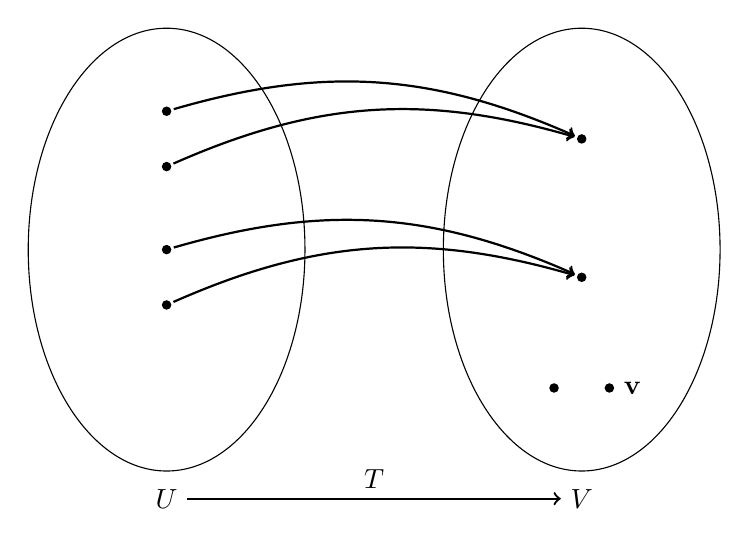
\begin{tikzpicture}
\tikzset{ltvect/.style={shape=circle, minimum size=0.30em, inner sep=0pt, draw, fill=black}}
\tikzset{ltedge/.style={->, bend left=20, thick, shorten <=0.1em, shorten >=0.1em}}
% base generic picture
\draw ( 5em, 8em) circle [x radius=5em, y radius=8em, thick];
\draw (20em, 8em) circle [x radius=5em, y radius=8em, thick];
\node (U) at ( 5em, -1em) {$U$};
\node (V) at (20em, -1em) {$V$};
\draw[->, thick, draw] (U) to node[auto] {$T$} (V);
% inputs
\node (u1) [ltvect]                         at (5em, 13em) {};
\node (u2) [ltvect]                         at (5em, 11em) {};
\node (u3) [ltvect]                         at (5em,  8em) {};
\node (u4) [ltvect]                         at (5em,  6em) {};
% outputs
\node (v1) [ltvect]                         at (20em, 12em) {};
\node (v2) [ltvect]                         at (20em,  7em) {};
\node (v3) [ltvect]                         at (19em,  3em) {};
\node (v)  [ltvect, label=right:$\vect{v}$] at (21em,  3em) {};
% associations
\draw[ltedge] (u1) to (v1);
\draw[ltedge] (u2) to (v1);
\draw[ltedge] (u3) to (v2);
\draw[ltedge] (u4) to (v2);
\end{tikzpicture}
\end{image}

To show that a linear transformation is not surjective, it is enough to find a single element of the codomain that is never created by any input, as in \ref{example:NSAQ}.  However, to show that a linear transformation is surjective we must establish that \textit{every} element of the codomain occurs as an output of the linear transformation for some appropriate input.


\begin{example}

Consider the linear transformation
\[
\ltdefn{T}{\complex{5}}{\complex{5}},\quad
\lteval{T}{\colvector{x_1\\x_2\\x_3\\x_4\\x_5}}=
\colvector{-65 x_1 + 128 x_2 + 10 x_3 - 262 x_4 + 40 x_5\\
36 x_1 - 73 x_2 - x_3 + 151 x_4 - 16 x_5\\
-44 x_1 + 88 x_2 + 5 x_3 - 180 x_4 + 24 x_5\\
34 x_1 - 68 x_2 - 3 x_3 + 140 x_4 - 18 x_5\\
12 x_1 - 24 x_2 - x_3 + 49 x_4 - 5 x_5}
\]


To establish that this transformation is surjective we must begin with a totally arbitrary element of the codomain, $\vect{v}$ and somehow find an input vector $\vect{u}$ such that $\lteval{T}{\vect{u}}=\vect{v}$.  We desire,
\begin{align*}
\lteval{T}{\vect{u}}&=\vect{v}\\
\colvector{-65 u_1 + 128 u_2 + 10 u_3 - 262 u_4 + 40 u_5\\
36 u_1 - 73 u_2 - u_3 + 151 u_4 - 16 u_5\\
-44 u_1 + 88 u_2 + 5 u_3 - 180 u_4 + 24 u_5\\
34 u_1 - 68 u_2 - 3 u_3 + 140 u_4 - 18 u_5\\
12 u_1 - 24 u_2 - u_3 + 49 u_4 - 5 u_5}
&=
\colvector{v_1\\v_2\\v_3\\v_4\\v_5}\\
\begin{bmatrix}
-65&128&10&-262&40\\
36&-73&-1&151&-16\\
-44&88&5&-180&24\\
34&-68&-3&140&-18\\
12&-24&-1&49&-5
\end{bmatrix}
\colvector{u_1\\u_2\\u_3\\u_4\\u_5}
&=
\colvector{v_1\\v_2\\v_3\\v_4\\v_5}
\end{align*}




We recognize this equation as a system of equations in the variables $u_i$, but our vector of constants contains symbols.  In general, we would have to row-reduce the augmented matrix by hand, due to the symbolic final column.  However, in this particular example, the $5\times 5$ coefficient matrix is nonsingular and so has an inverse (\ref{theorem:NI}, \ref{definition:MI}).
\[
\inverse{
\begin{bmatrix}
-65&128&10&-262&40\\
36&-73&-1&151&-16\\
-44&88&5&-180&24\\
34&-68&-3&140&-18\\
12&-24&-1&49&-5
\end{bmatrix}
}
=
\begin{bmatrix}
-47 & 92 &  1 & -181 & -14 \\
 27 & -55 & \frac{7}{2} & \frac{221}{2} & 11\\
-32 & 64  & -1 &  -126 &  -12\\
 25 &  -50 &  \frac{3}{2} & \frac{199}{2} & 9 \\
 9 & -18 & \frac{1}{2} & \frac{71}{2} & 4
\end{bmatrix}
\]
so we find that
\begin{align*}
\colvector{u_1\\u_2\\u_3\\u_4\\u_5}
&=
\begin{bmatrix}
-47 & 92 &  1 & -181 & -14 \\
 27 & -55 & \frac{7}{2} & \frac{221}{2} & 11\\
-32 & 64  & -1 &  -126 &  -12\\
 25 &  -50 &  \frac{3}{2} & \frac{199}{2} & 9 \\
 9 & -18 & \frac{1}{2} & \frac{71}{2} & 4
\end{bmatrix}
\colvector{v_1\\v_2\\v_3\\v_4\\v_5}\\
&=
\colvector{-47 v_1 + 92 v_2 + v_3 - 181 v_4 - 14 v_5\\
 27 v_1 - 55 v_2 + \frac{7}{2} v_3 + \frac{221}{2} v_4  + 11 v_5\\
-32 v_1 + 64  v_2 - v_3 - 126 v_4 - 12 v_5\\
 25 v_1 - 50 v_2 + \frac{3}{2} v_3 + \frac{199}{2} v_4 + 9 v_5\\
 9 v_1 - 18 v_2 + \frac{1}{2} v_3 + \frac{71}{2} v_4 + 4 v_5}
\end{align*}


This establishes that if we are given \textit{any} output vector $\vect{v}$, we can use its components in this final expression to formulate a vector $\vect{u}$ such that $\lteval{T}{\vect{u}}=\vect{v}$.  So by \ref{definition:SLT} we now know that $T$ is surjective.  You might try to verify this condition in its full generality (i.e.,  evaluate $T$ with this final expression and see if you get $\vect{v}$ as the result), or test it more specifically for some numerical vector $\vect{v}$.

\end{example}

Here is the cartoon for a surjective linear transformation.  It is meant to suggest that for every output in $V$ there is <em>at least one</em> input in $U$ that is sent to the output.  (Even though we have depicted several inputs sent to each output.)  The key feature of this cartoon is that there are no vectors in $V$ without an arrow pointing to them.
\begin{image}
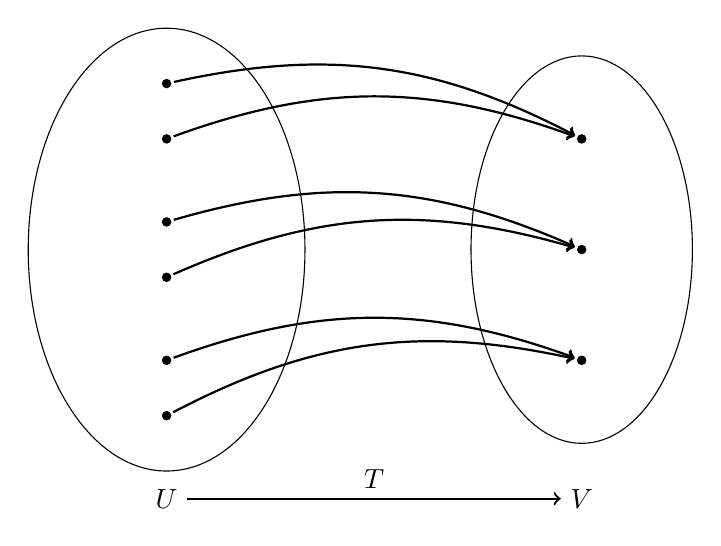
\begin{tikzpicture}
\tikzset{ltvect/.style={shape=circle, minimum size=0.30em, inner sep=0pt, draw, fill=black}}
\tikzset{ltedge/.style={->, bend left=20, thick, shorten <=0.1em, shorten >=0.1em}}
% base generic picture
\draw ( 5em, 8em) circle [x radius=5em, y radius=8em, thick];
\draw (20em, 8em) circle [x radius=4em, y radius=7em, thick];
\node (U) at ( 5em, -1em) {$U$};
\node (V) at (20em, -1em) {$V$};
\draw[->, thick, draw] (U) to node[auto] {$T$} (V);
% inputs
\node (u1) [ltvect]                         at (5em, 14em) {};
\node (u2) [ltvect]                         at (5em, 12em) {};
\node (u3) [ltvect]                         at (5em,  9em) {};
\node (u4) [ltvect]                         at (5em,  7em) {};
\node (u5) [ltvect]                         at (5em,  4em) {};
\node (u6) [ltvect]                         at (5em,  2em) {};
% outputs
\node (v1) [ltvect]                         at (20em, 12em) {};
\node (v2) [ltvect]                         at (20em,  8em) {};
\node (v3) [ltvect]                         at (20em,  4em) {};
% associations
\draw[ltedge] (u1) to (v1);
\draw[ltedge] (u2) to (v1);
\draw[ltedge] (u3) to (v2);
\draw[ltedge] (u4) to (v2);
\draw[ltedge] (u5) to (v3);
\draw[ltedge] (u6) to (v3);
\end{tikzpicture}
\end{image}

Let us now examine a surjective linear transformation between abstract vector spaces.

\begin{example}
Consider
\[\ltdefn{T}{P_3}{M_{22}},\quad\lteval{T}{a+bx+cx^2+dx^3}=
\begin{bmatrix}
a+b & a-2c\\
d & b-d
\end{bmatrix}
\]

Begin by choosing an arbitrary output.  In this example, we need to choose an arbitrary $2\times 2$ matrix, say
\[
\vect{v}=\begin{bmatrix}x&y\\z&w\end{bmatrix}
\]
and we would like to find an input polynomial
\[
\vect{u}=a+bx+cx^2+dx^3
\]
so that $\lteval{T}{\vect{u}}=\vect{v}$.  So we have,
\begin{align*}
\begin{bmatrix}x&y\\z&w\end{bmatrix}&=\vect{v}\\
&=\lteval{T}{\vect{u}}\\
&=\lteval{T}{a+bx+cx^2+dx^3}\\
&=\begin{bmatrix}
a+b & a-2c\\
d & b-d
\end{bmatrix}
\end{align*}




Matrix equality leads us to the system of four equations in the four unknowns, $x,y,z,w$,
\begin{align*}
a+b&=x\\
a-2c&=y\\
d&=z\\
b-d&=w
\end{align*}
which can be rewritten as a matrix equation,
\[
\begin{bmatrix}
1 & 1 & 0 & 0\\
1 & 0 & -2 & 0 \\
0 & 0 & 0 & 1\\
0 & 1 & 0 & -1
\end{bmatrix}
\colvector{a\\b\\c\\d}
=
\colvector{x\\y\\z\\w}
\]




The coefficient matrix is nonsingular, hence it has an inverse,
\[
\inverse{
\begin{bmatrix}
1 & 1 & 0 & 0\\
1 & 0 & -2 & 0 \\
0 & 0 & 0 & 1\\
0 & 1 & 0 & -1
\end{bmatrix}
}
=
\begin{bmatrix}
1 & 0 & -1 & -1\\
0 & 0 & 1 & 1\\
\frac{1}{2} & -\frac{1}{2} & -\frac{1}{2} & -\frac{1}{2}\\
0 & 0 & 1 & 0
\end{bmatrix}
\]
so we have
\begin{align*}
\colvector{a\\b\\c\\d}&=
\begin{bmatrix}
1 & 0 & -1 & -1\\
0 & 0 & 1 & 1\\
\frac{1}{2} & -\frac{1}{2} & -\frac{1}{2} & -\frac{1}{2}\\
0 & 0 & 1 & 0
\end{bmatrix}
\colvector{x\\y\\z\\w}\\%
&=
\colvector{
x-z-w\\
z+w\\
\frac{1}{2}(x-y-z-w)\\
z
}
\end{align*}




So the input polynomial $\vect{u}=(x-z-w)+(z+w)x+\frac{1}{2}(x-y-z-w)x^2+zx^3$ will yield the output matrix $\vect{v}$, no matter what form $\vect{v}$ takes.  This means by \ref{definition:SLT} that\ldots
\begin{multipleChoice}
\choice[correct]{$T$ is surjective.}
\choice{$T$ is not surjective.}
\end{multipleChoice}

  All the same, let us do a concrete demonstration and evaluate $T$ with $\vect{u}$,
\begin{align*}
\lteval{T}{\vect{u}}&=\lteval{T}{(x-z-w)+(z+w)x+\frac{1}{2}(x-y-z-w)x^2+zx^3}\\
&=
\begin{bmatrix}
(x-z-w)+(z+w) & (x-z-w) - 2(\frac{1}{2}(x-y-z-w))\\
z & (z+w)-z
\end{bmatrix}\\
&=
\begin{bmatrix}
x & y\\
z & w
\end{bmatrix}\\
&=\vect{v}
\end{align*}




\end{example}
\end{document}


%%% Local Variables:
%%% mode: latex
%%% TeX-master: t
%%% End:
